\section{FedITN}

\begin{frame}{Project definition}
  \begin{block}{Objective}
  Design a systematic approach to generate \emph<+>{deployable} network topologies, capable of producing \emph<+>{heterogeneous} and \emph<+>{independent} datasets for evaluating Federated Intrusion Detection Systems (FIDSs).
  \end{block}

  \pause
  \begin{block}{Requirements}
    \begin{itemize}[<+->]
      \item \emph{diversity} in topologies, attacks and devices to provide heterogeneity;
      \item approach \emph{realism} in terms of traffic and behaviors;
      \item \emph{controllable} data distribution across clients;
      \item data \emph{independence} amongst clients;
    \end{itemize}
  \end{block}
\end{frame}

% \begin{frame}{Related work}
%   \begin{columns}[t]
%     \begin{column}{.33\textwidth}
%       \begin{block}{Protocol testing~\autocite{doar_bettermodelgenerating_1996,medina_BRITEapproachuniversal_2001}}
%         \begin{itemize}
%           \item Internet-like topologies, not applicable to enterprise networks;
%           \item focus on structural properties or degree distributions (\eg, power-law).
%         \end{itemize}
%       \end{block}
%     \end{column}
%     \onslide<+(1)->
%     \begin{column}{.33\textwidth}
%       \begin{block}{Usecase or task focused}
%         \begin{itemize}[<+->]
%           \item Declarative topology generation (\eg, \texttt{TopoGen}~\autocite{laurito_TopoGennetworktopology_2017} for SDN);
%           \item Layer-based composition for Industrial Control Networks (\eg, \texttt{GENIND}~\autocite{alrumaih_GENINDindustrialnetwork_2023});
%         \end{itemize}
%       \end{block}
%     \end{column}
    
%     \onslide<.(1)->
%     \begin{column}{.33\textwidth}
%       \begin{block}{Cyber-ranges}
%         \begin{itemize}[<+->]
%           \item Declarative deployments of scenarios and topologies~\autocite{venkatesan_VulnerVANVulnerableNetwork_2019,yamin_Modelingexecutingcyber_2022};
%           \item Vulnerable environment generation from attack graphs (\eg, \texttt{URSID}~\autocite{besson_URSIDAutomaticallyRefining_2024a}).
%         \end{itemize}
%       \end{block}
%     \end{column}
%   \end{columns}

%   \only<1>{\footcite*{doar_bettermodelgenerating_1996,medina_BRITEapproachuniversal_2001}}
%   \only<2-3>{\footcite*{laurito_TopoGennetworktopology_2017}}
%   \alt<3>{\footcite*{alrumaih_GENINDindustrialnetwork_2023}}{\only<2>{\blankfootnote{}\blankfootnote{}}}
%   \only<4-5>{\footcite*{venkatesan_VulnerVANVulnerableNetwork_2019}}
%   \alt<5>{\footcite*{yamin_Modelingexecutingcyber_2022}}{\only<4>{\blankfootnote{}\blankfootnote{}}}
  

% \end{frame}

\begin{frame}{FedITN Approach Overview}
  % attack scenarios -> constraints -> compatible subtopologies -> topology trees
  \centering
  \includegraphics<1>[width=.9\textwidth]{figures/feditn/approach/overview-1}%
  \includegraphics<2>[width=.9\textwidth]{figures/feditn/approach/overview-2}%
\end{frame}

\begin{frame}{Topology composition}
  \centering
  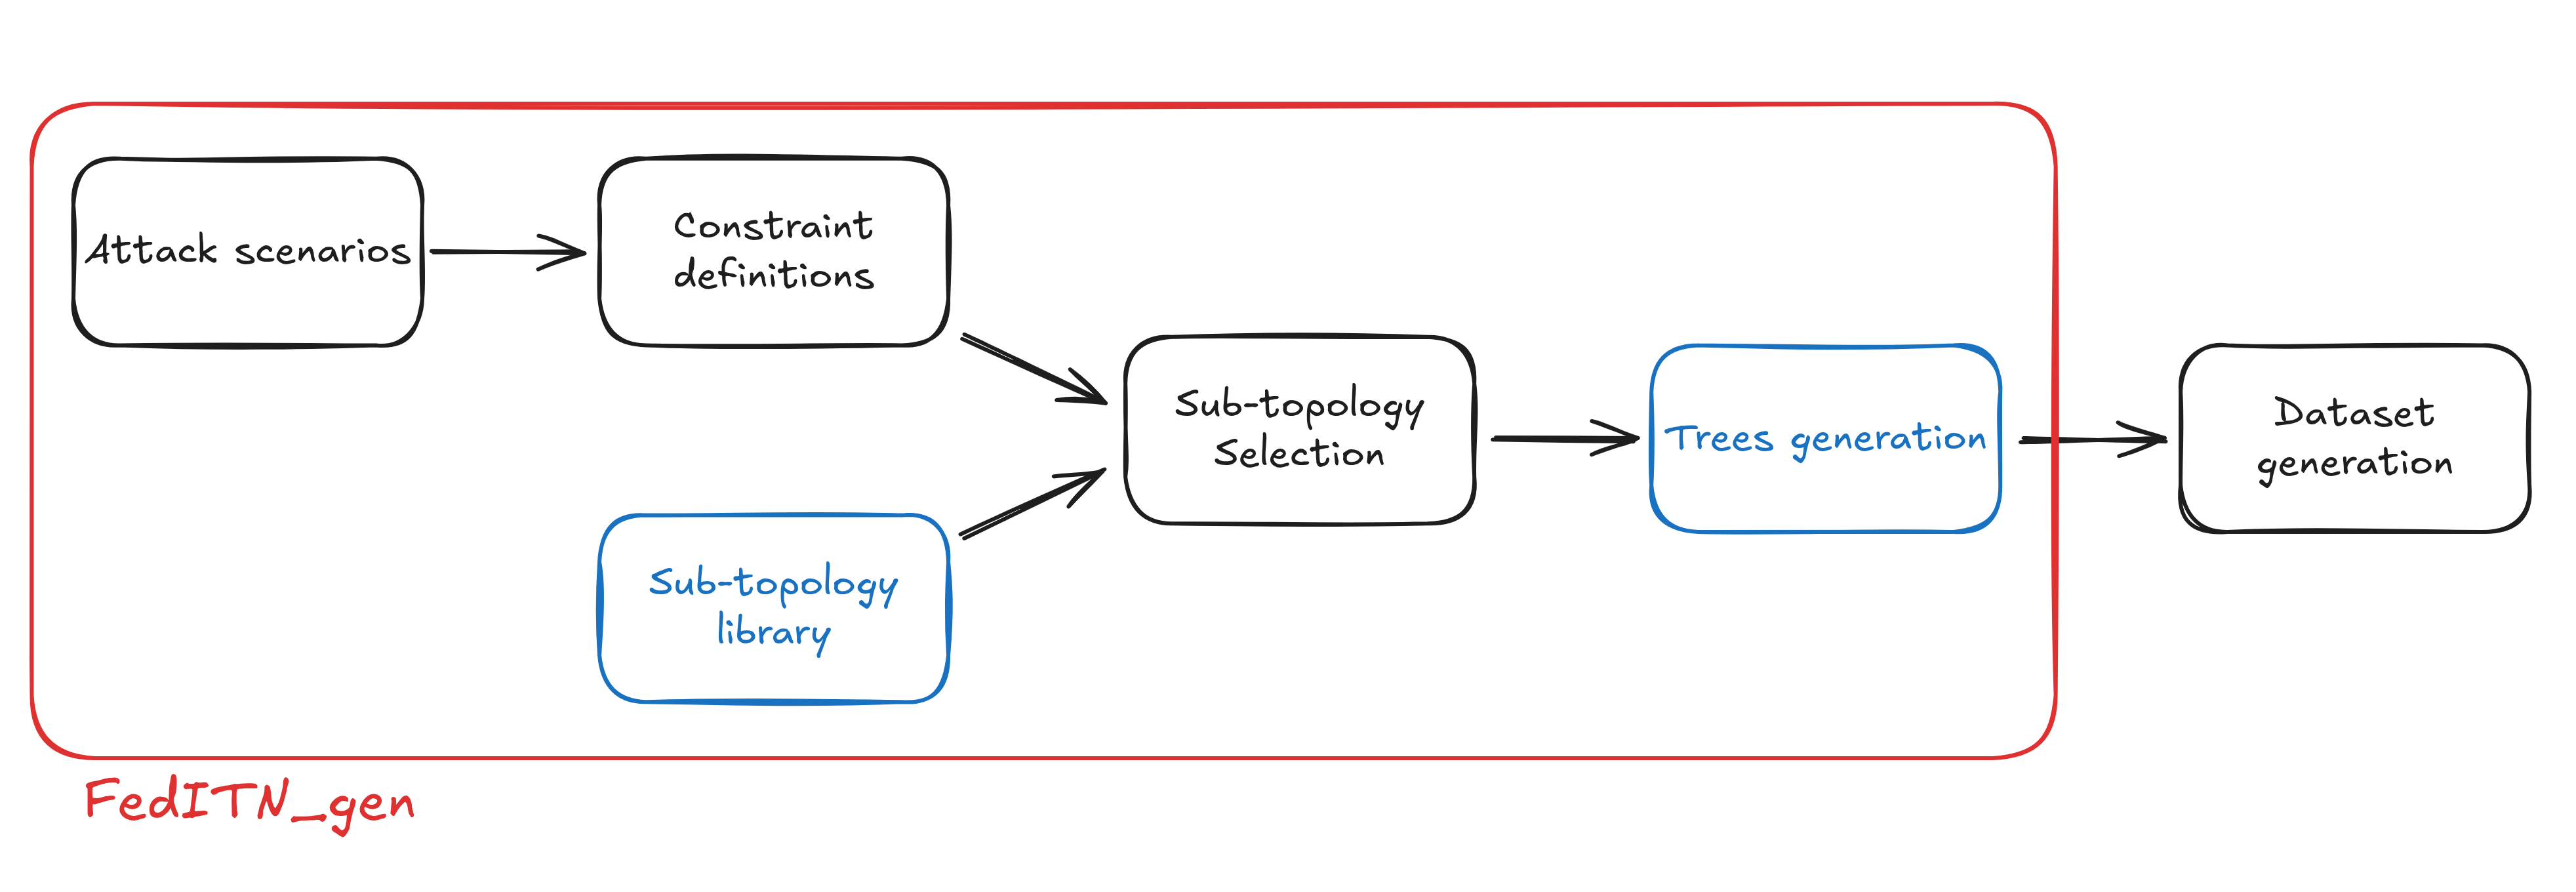
\includegraphics[width=.9\textwidth]{figures/feditn/approach/overview-topo}
\end{frame}

\begin{frame}{Sub-topologies}
  \begin{columns}
    \begin{column}{0.4\textwidth}
      \begin{figure}
        \centering
        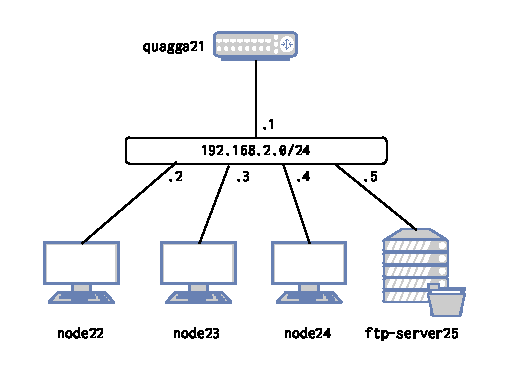
\includegraphics[width=\linewidth]{figures/feditn/approach/sub_topology.pdf}
        \caption{Example of a sub-topology with 2 types of nodes.}
      \end{figure}
    \end{column}

    \begin{column}{0.6\textwidth}
      \begin{block}{Sub-topologies}
        \begin{itemize}[<+->]
          \item Reusable building blocks;
          \item Each sub-topology has a specific role and properties (\eg, services\footnotemark, vulnerabilities);
          \item the router acts as a gateway between sub-topologies.
        \end{itemize}
      \end{block}
        
      \pause
      \begin{block}{Composition}
        \begin{itemize}[<+->]
          \item Sub-topologies are connected to form a tree (to avoid cycles);
          \item automatic routing with OSPF;
          \item the \texttt{Master} sub-topology contains the Internet gateway, the main DNS server, and DHCP/OSPF services.
        \end{itemize}
      \end{block}
    \end{column}
  \end{columns}
  \alt<2->{\footnotetext{Available services: \texttt{ldap}, \texttt{dbms}, \texttt{cms}, \texttt{dns}, \texttt{mail}, \texttt{syslog\_server}, \texttt{web}, \texttt{ftp}, \texttt{proxy}, \texttt{cloud\_storage}.}}{\only<1>{\blankfootnote{}}}

\end{frame}

\begin{frame}
  \begin{figure}
    \centering
    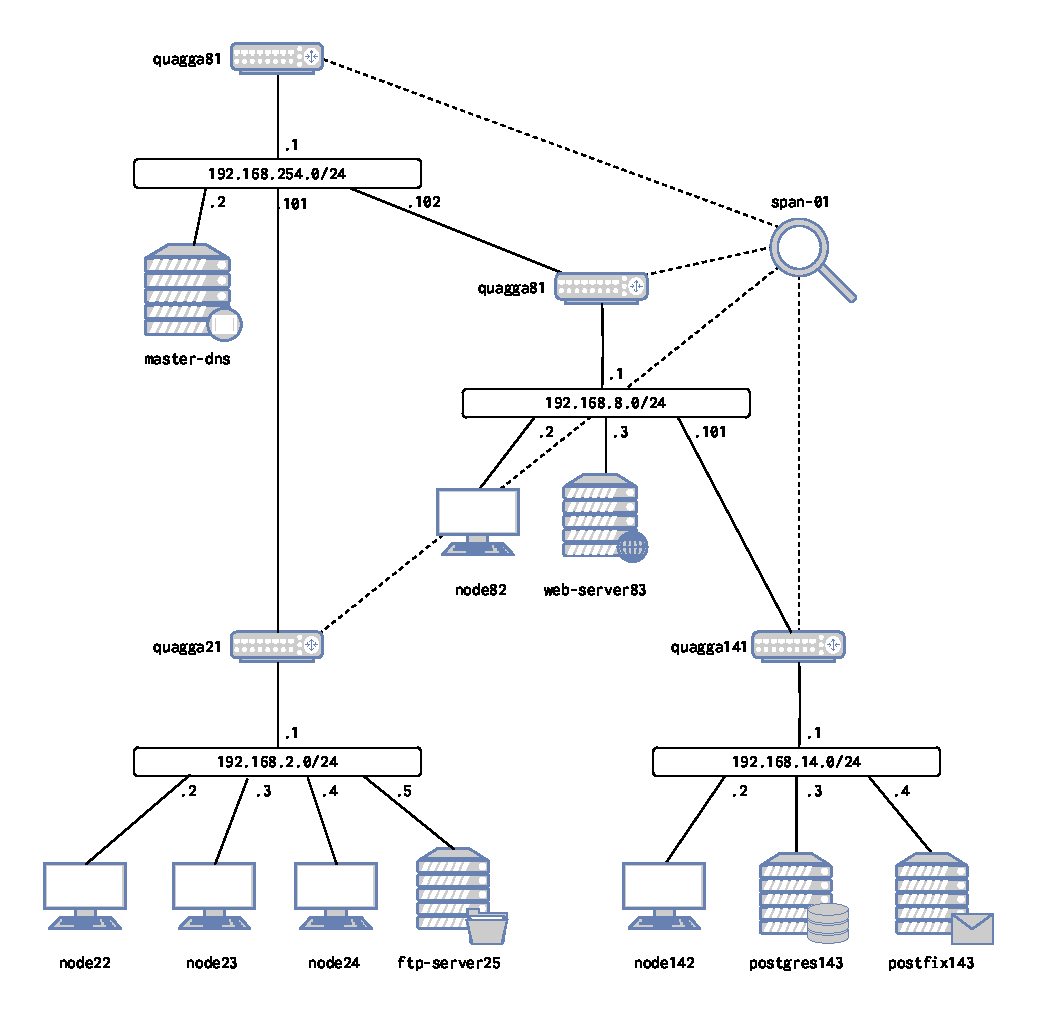
\includegraphics[height=\paperheight]{figures/feditn/approach/topology.pdf}
    \caption{Example of a generated topology with 3 sub-topologies.}
  \end{figure}
\end{frame}

      



\begin{frame}{Attack Scenarios}
  \centering
  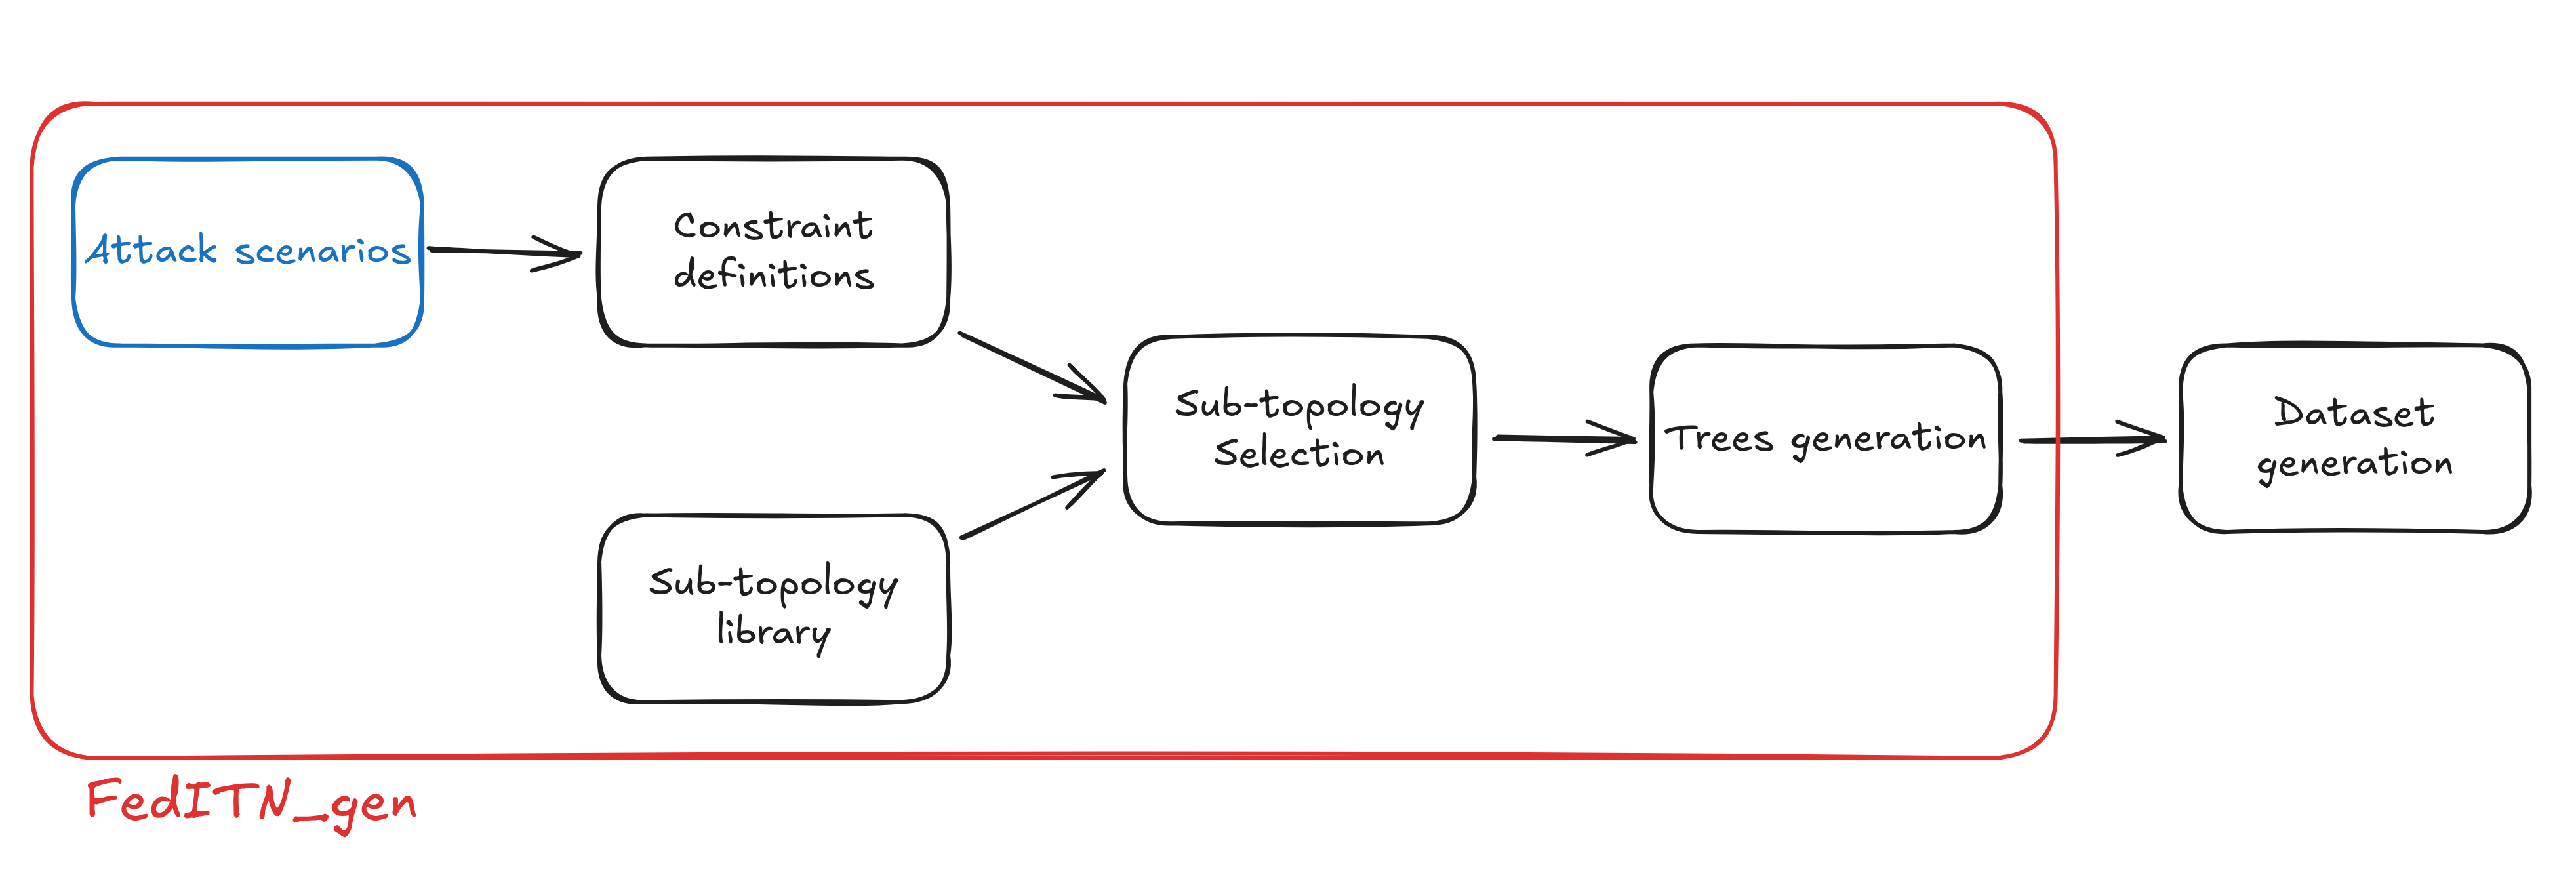
\includegraphics[width=.9\textwidth]{figures/feditn/approach/overview-attack}
\end{frame}

\begin{frame}[standout]
  \foreach \i in {1,2} {%
    \includegraphics<\i>[height=\paperheight]{figures/feditn/approach/scenario-\i}%
  }
\end{frame}


\begin{frame}{Constraint Programming}
  \centering
  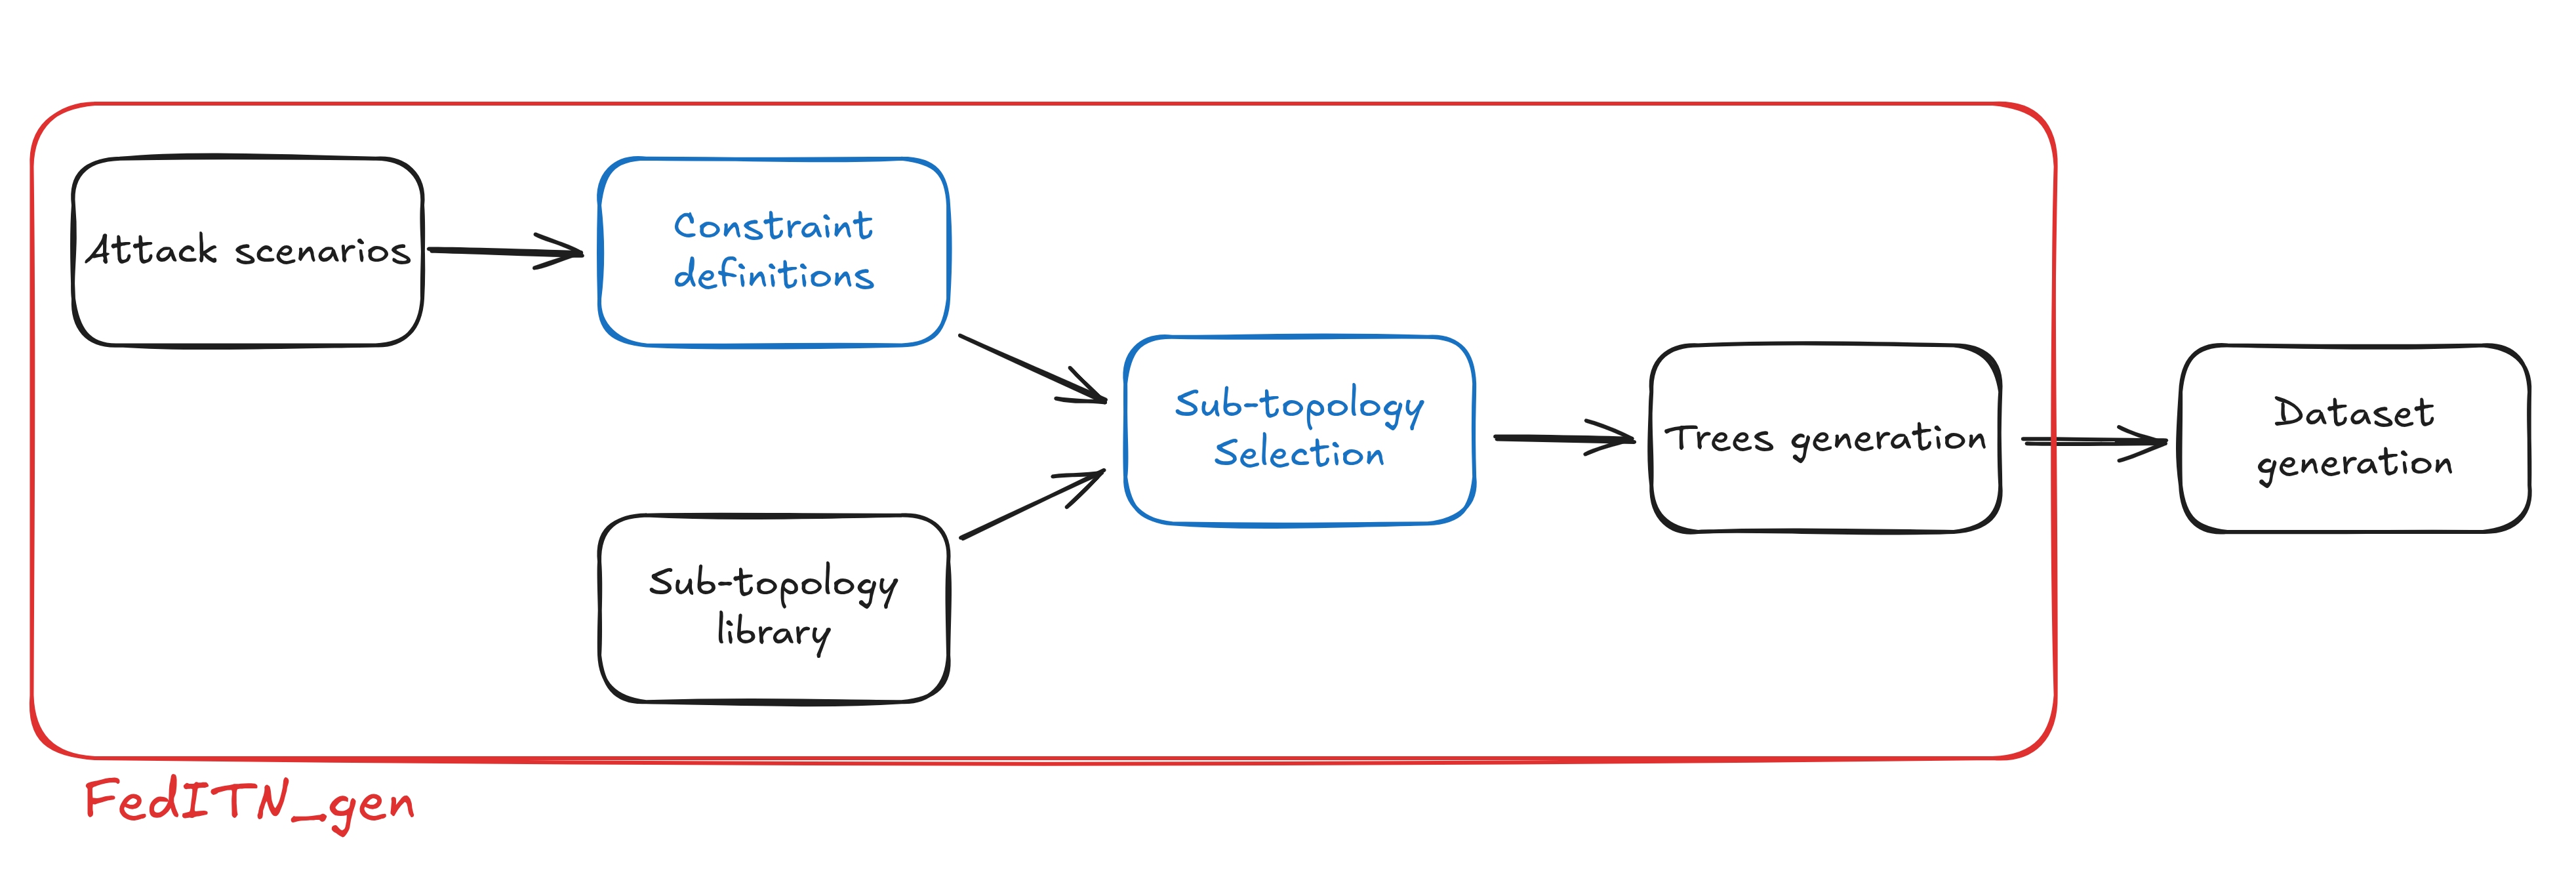
\includegraphics[width=.9\textwidth]{figures/feditn/approach/overview-constraint}
\end{frame}

\begin{frame}{Problem Formalization}
\begin{block}{Sub-topology Selection Problem (STSP)}
  \color<2->{black!30}
  Let $\mathcal{T} = \{\tau_1, \tau_2, \ldots, \tau_n\}$ be a set of sub-topologies, \alert<4>{$D_\text{service}$ a set of services}, \alert<5>{$A = \{a_1, a_2, \ldots, a_m\}$ a set of attack scenarios}, \alert<2>{$k_\text{min}$ and $k_\text{max}$ the bounds of the number of subtopologies}, and \alert<3>{$\ell_\text{min}$ and $\ell_\text{max}$ the bounds for the total number of nodes}.
  The STSP consists of finding all sets of sub-topologies $T \subseteq \mathcal{T}$ that satisfy the following:
  \begin{enumerate}
    \color<2->{black!30}
    %\normalfont
    \item \alert<2>{$k_\text{min} \leq |T|  \leq k_\text{max}$}.
    \item \alert<3>{$\ell_\text{min} \leq \sum\nolimits_{\tau_k \in T} | N_k| \leq \ell_\text{max}$}.
    \item \alert<4>{$\forall s \in D_\text{service}, \exists \tau_k \in T, \text{ s.t. } s \in N_k$}.
    \item \alert<5>{$\forall a \in A, \forall s \in a_{[\texttt{srcs}]}, \exists \tau_k \in T, \text{ s.t. } s \text{ compatible with } \tau_k$}.
    \item \alert<5>{$\forall a \in A, \forall t \in a_{[\texttt{targets}]}, \exists \tau_k \in T, \text{ s.t. } t \text{ compatible with } \tau_k$}.
  \end{enumerate}
\end{block}
    
\end{frame}

\begin{frame}{Selection \& Composition}
  \begin{block}{Solution search}
    \begin{itemize}[<+->]
      \item Use of the CP-SAT solver from Google OR-Tools~\footnote{https://developers.google.com/optimization};
      \item The solver finds all combinations of sub-topologies satisfying the constraints;
      \item Incompatible services are pruned during the search.
      \item Trees are generated with backtracking to respect an additional depth constraint.
    \end{itemize}
  \end{block}

  \onslide<.>{\begin{figure}
    \centering
    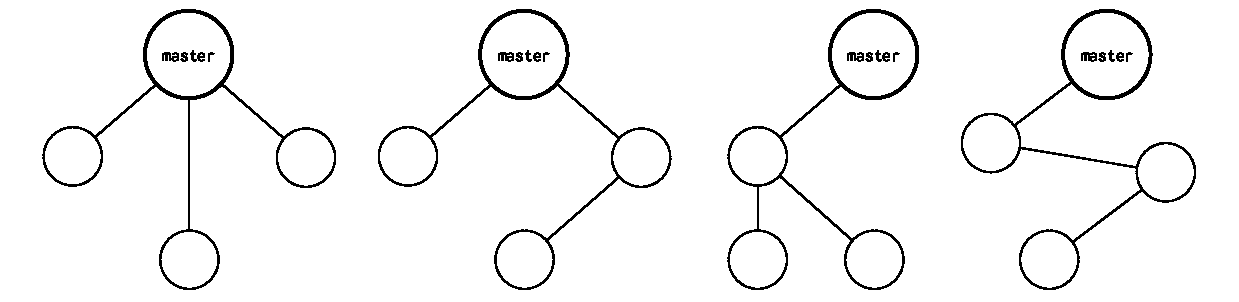
\includegraphics[width=.9\textwidth]{figures/feditn/approach/trees-3}
    \caption{Possible tree arrangements for 3 sub-topologies.}
  \end{figure}}

\end{frame}